\documentclass[../main.tex]{subfiles}
\graphicspath{{\subfix{../../Images}}}

\begin{document}
\section{Cadence-Flow NFT Implementation Details}
\label{sec:cadence_flow_nft_implementation}
Flow's version of the ERC721 standard is simply named the \textit{NonFungibleToken} standard and is defined by a contract interface file with same name, specifically, the importable \verb|NonFungibleToken.cdc| file. Contract interfaces in Flow/Cadence work very similarly to the ones in Ethereum/Solidity: these files define a set of default functions, internal parameters, events and resources, the latter replacing Ethereum's mappings, though in functionally different manner.
\par
The implementation of the Flow/Cadence NFT example was as similar as possible to the Ethereum implementation from Sec. \ref{sec:solidity_ethereum_nft_implementation}, towards providing the most objective comparison possible. In this sense, the Cadence NFT was implemented following the corresponding Flow standard to Ethereum's ERC721, namely the \textit{NonFungibleToken} standard, and an auxiliary standard used to extend token functionalities, namely the \textit{MetadataViews} standard, which provides similar functionalities to the ERC721URIStorage imported in the Ethereum solution.
\par
Flow's version of the NFT contract distributes token functionalities in two levels: the contract itself and the resource(s) used to implement NFT mechanics. As such, representing this contract with a similar approach to the one taken for Fig. \ref{fig:solidity_contract_architecture} results in a confusing scheme. To address this, we split the organization of the contract through the levels indicated:

\begin{figure}[htp]
    \centering
    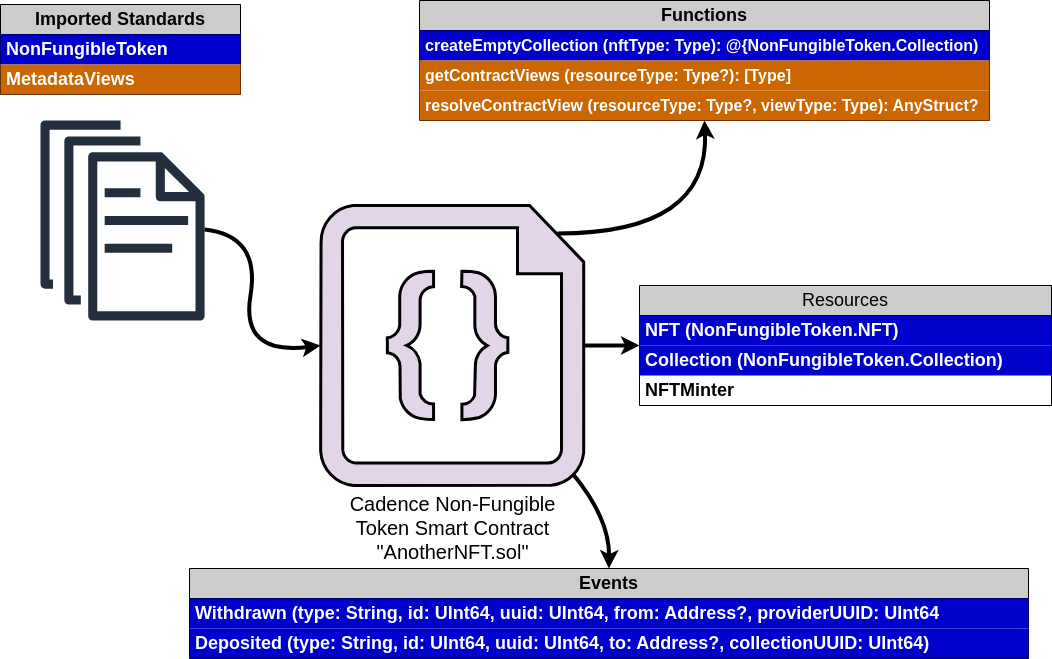
\includegraphics[width=0.7\textwidth]{../Images/05_Cadence_NFT_Contract_Arch.png}
    \caption{General organisation of a Cadence NFT minting contract}
    \label{fig:cadence_contract_architecture}
\end{figure}

Fig \ref{fig:cadence_contract_architecture} provides a generalist view of the NFT implementing contract. The main difference from the Solidity approach is the usage of \textit{resources} instead of \textit{mappings}. Other than this, the Ethereum and Flow NFT standards are quite similar, though resources are functionally more complex than mappings, thus the correspondence between these two concepts is not necessarily symmetrical even though both are used to implement token ownership in their respective blockchains.
\par
Given the added complexity brought by Flow's usage of resources, Fig. \ref{fig:cadence_nft_architecture} and Fig. \ref{fig:cadence_collection_architecture} provide overviews of the two resources that require implementation due to the standardisation of the contract.

\subsection{Cadence Types}
\label{sec:cadence_types}
Cadence is a type-safe language. Every data element in Cadence has a type, including complex elements such as resources and struts. Cadence relies in type matching as means to ensure data integrity in blockchain operations. Complex types are defined by the name of the contract that define them concatenated with the name of the resource. For example, if smart contract \textbf{ContractA} defines a resource named \textbf{ResourceA}, they type of each instance of this resource is \textbf{ContractA.ResourceA}.

\subsection{Contract defined Resources}
In Flow, Non-Fungible Tokens are digital objects, defined very similarly to objects in \textit{Object-Oriented Programming} language, such as Java, Python, C\#, etc., except that resources are limited to exist in one location at a time, cannot be copied, etc. The definition of a basic Non-Fungible Token digital object is shown in Fig. \ref{fig:cadence_nft_architecture}. In its simplest form, a \textit{NonFungibleToken} compliant resource requires just an id.
\par
The Cadence implementation is objectively more complex than the Ethereum one, based on how more complicated Flow's storage architecture is compared to Ethereum. While it was possible to represent Ethereum's NFT architecture in one figure, the same exercise for the Cadence version requires more detail to be properly understood. Cadence smart contracts define NFTs as a resource but they also typically define an adjacent resource, usually in the same NFT contract, named \textit{Collection}.
\par
In simple terms, a Collection is a resource that can store other resources. Collection are used to simplify the storage of multiple tokens into a single user account. In Flow tokens are saved to a logic path in an account's storage area, as it was referred in Sec. \ref{sec:storage_in_flow}, that needs to be unique for every resource in storage. In other words, it is not possible to save two resources to the same storage path, just like an operating system cannot save two files to the same file path (the underlying principle is the same). This limitation can exponentially complicate storage of multiple objects, since each requires a new storage path different from the other ones.
\par
Collections solve this by enabling the storage of multiple digital objects in the same collection, as long as they share the same type, thus requiring only one unique storage path for the collection itself. In the operating system analogy, collections are akin to directories that contain multiple files. The storage intricacies of Flow make collections almost indispensable to organise the storage of resources, and as such these were included in the NonFungibleToken standard as well.
\par
The NFT smart contract created for this purpose, whose architecture is depicted in Fig. \ref{fig:cadence_contract_architecture}, defines three resources: the NFT itself, a NFT minter and a Collection. The NFT and the Collection were defined according to the specifications derived from the NonFungibleToken standard and, as such, their type (indicated inside the parenthesis) derives from the standard itself. Sec. \ref{sec:cadence_types} goes into detail about Cadence use of types.
\par
The NFTMinter is a non standardised resource that is used to simplify the minting of new NFT resources while able to maintain access to this functionality to the deployer/owner of the smart contract, as well as extending it to other users if required. New NFTs are created using the \textbf{create} keyword in a transaction (creating resources changes the state of the blockchain, therefore they cannot happen in scripts) but this operation is restricted by default to the owner of the contract, i.e, the owner of the account that contains the contract in storage. Wrapping this process in a resource, the NFTMinter, provides several advantages:

\begin{itemize}
    \item{Simplifies the creation of new NFTs} by abstracting it to a function call from the NFTMinter resource.
    \item {Provides a easy methods to delegate access} by creating a publishing capabilities that can be used to delegate the creation of new NFTs to other, authorised, users.
    \item {Increased flexibility} towards additional logic to execute before creating the new resource. The function that returns the new NFT resource can be edited to include additional validations, access control, etc.
\end{itemize}

The NFTMinter is not a standardised resource, therefore its type is actually \textit{ExampleNFT.NFTMinter} because its definition exists only in the contract named \verb|ExampleNFT.cdc|. Since the minter is not part of any of the standards included, including one in a NFT contract is considered a good programming practice in Cadence rather than a critical resource, given that it is possible to create new NFTs without it.

\subsubsection{Functions}
\label{sec:flow_contract_functions}
The majority of the NFT mechanics are abstracted by the NFT resource itself, which leaves little else requiring implementation from the imported standards. The NonFungibleToken requires only a function to create empty Collections. At the contract level, this function requires a type to be provided a priori, which "locks" the collection created to accept only resources from the provided type. The remaining functions, \textit{getContractViews} and \textit{resolveContractView} are required by the MetadataViews standard and are used mainly to process token metadata. Since we do not intend to use them in this exercise, these were implemented as stubs.
\par
The only function required from the NonFungibleToken standard is the \textit{createEmptyCollection}, which returns a resource with the type \textit{NonFungibleToken.Collection}. The '@' in the function signature indicates that the function returns a resource with the type that follows that symbol. Because this invocation occurs at the contract level, the function requires the user to provide the type of resource that is to be stored in the collection, since this is a standardised function and as such cannot infer a priori the types of resources inferable from the contract.

\subsubsection{Events}
\label{sec:flow_contract_events}
The standards define the events to emit during token transactions at the contract level. Cadence requires an explicit declaration of all the elements indicated in Fig. \ref{fig:cadence_contract_architecture} except the events. These are inherited by default by importing the NonFungibleToken contract interface. The \textit{withdraw} and \textit{deposit} functions are implemented in the collection resource and the standard already includes the automatic emission of these events.


\subsection{Non-Fungible Token Resource}
This is the main resource in this contract. Fig. \ref{fig:cadence_nft_architecture} presents a architecture scheme for the implementation of the NFT resource itself. This definition is part of the contract file but as a digital object, resources are significantly complex than mappings and as such deserve to be explored in detail. The ownership of each NFT in Flow is ensured by the ownership mechanism established by the blockchain, summarised by Fig. \ref{fig:flow_account}. Essentially, in Flow every resource needs to be "somewhere" at all times, and that implies that, at some point, resources can only exist in storage. The owner of an account that stores a NFT is also the owner of the token as well.

\begin{figure}[htp]
    \centering
    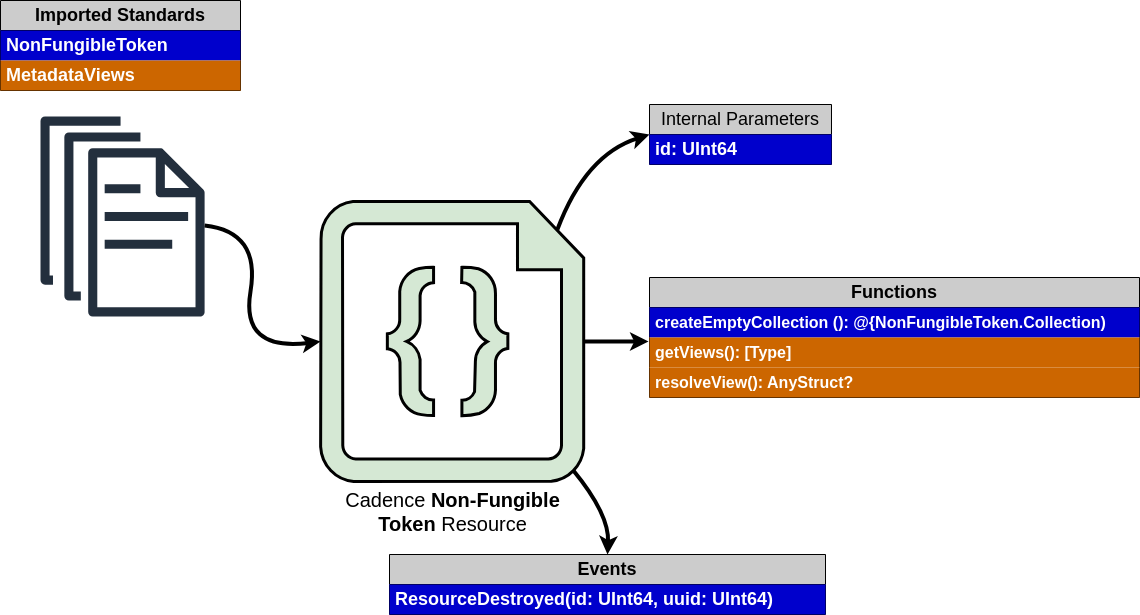
\includegraphics[width=0.7\textwidth]{../Images/06_Cadence_NFT_Arch.png}
    \caption{Organisation of a Non-Fungible Token resource in Flow}
    \label{fig:cadence_nft_architecture}
\end{figure}

We defined the simplest NFT possible in Cadence, which consists in its unique id, a 64-bit unsigned integer, three functions that require implementation by the standard imports from the parent contract, and a event that is automatically emitted if a resource of the type of this NFT implementation, i.e., an instance of this NFT, is destroyed. Owners of resources can destroy them with the \textbf{destroy} keyword, by either invoking a contract function that does it, or running a transaction that executes this command on an owned resource. It is important to note that destroying a NFT resource in Cadence with the \textbf{destroy} command is different than \textit{burning} the token, which consists in transferring the resource to an unrecoverable address, as it is custom in other blockchain such as Ethereum. Flow has \textit{Burner} contract that implements a \textit{Burnable} interface which exposes a \textit{burn} function. This function replicates Ethereum's burning standard by validating extensively the ownership of the token against the address that is invoking the function, but, if all validations are passed, the resource is ultimately destroyed as in deleted from the storage space where it was saved. Destroying a NonFungibleToken-standardised NFT in Flow emits the \textit{ResourceDestroyed} event with the id of the token in question.
\par
Function-wise, the resource required a triple of functions very similar to the requirements from the parent contract. The MetadataViews-derived function relate to the processing of the metadata of the individual resource. They also have no direct correspondence to the Ethereum version and therefore were implemented as stubs also. Finally, this resource also implements a version for the \textit{createEmptyCollection} but this one, unlike the parent version from Sec. \ref{sec:flow_contract_functions}, is called from within the resource it is supposed to store. The collection resource returned from this version is already set to receive tokens with type \textit{NonFungibleToken.NFT}.

\subsection{Collection Resource}
Collections use a \textit{dictionary}, a structure used to store key-value pairs, thus similar to mappings in Ethereum. But in Cadence, dictionaries can hold resources as well. The standard imposed the use of the \textit{ownedNFTs} dictionary to pair the id of a token with the token resource itself as value. Though collections are not restricted to save a single type of resources, this cannot violate the fact that dictionaries must have unique keys and thus cannot store tokens with the same id, even if they have different types.

\begin{figure}[htp]
    \centering
    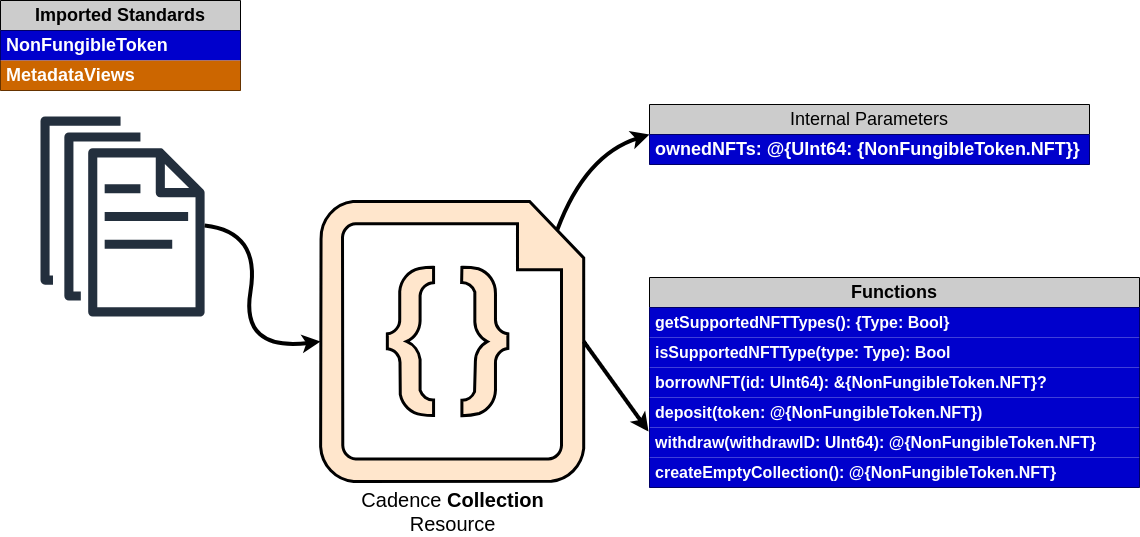
\includegraphics[width=0.7\textwidth]{../Images/07_Cadence_Collection_Arch.png}
    \caption{Organisation of a Collection resource in Flow}
    \label{fig:cadence_collection_architecture}
\end{figure}

Data integrity in collections is validated with the \textit{getSupportedNFTTypes} and \textit{isSupportedType} function. These function are available for external use but they are used internally to validate if a token with a non supported type is submitted to storage.
\par
Token transfer mechanics are abstracted and simplified by a pair of default functions from standardised collection resources, namely, \textit{deposit} and \textit{withdraw}. Resources are saved and loaded from storage using \textit{save} and \textit{load} functions from \textit{account} objects authorised to manipulate the respective account storage. This is the process to save collection resources to an account's storage, normally implemented with a transaction. But once a collection is available from storage, further stores of other resources, most usually NFTs, is simplified by calling the respective function from the collection resource itself. \textit{Deposit} requires a token provided as argument and does not return a value, \textit{withdraw} requires the id of the token to retrieve and returns the resource. Cadence's version of Solidity's \textit{transfer} function is split into a pair of function covering both directions of a transfer operation. Both functions emit the \textit{Deposited} and \textit{Withdrawn} indicated in Sec. \ref{sec:flow_contract_events} respectively.
\par
Flow allows users to retrieve data from a NFT resource saved in another user's account without even getting control of the resource itself by "borrowing" a reference to a token in storage instead of the resource itself. A \textit{resource} in Cadence works similar to a memory pointer retrievable to a resource saved in a different storage area. The \textit{borrowNFT} function can be customised to control which parameters and functions of the original resource are returned in the reference, thus allowing for granular access control to the resource without relinquishing its ownership. This is particularly useful to read metadata fields.
\par
Finally, the collection resource itself also includes yet another version of the \textit{createEmptyCollection} function, this one also configured with the \textit{NonFungibleToken.NFT} type as supported type for storage, since any invocation of this function also comes from within another collection resource already configured in this sense. This may seem redundant but it essentially provides these resources with a cloning functionality of sorts.
\end{document}